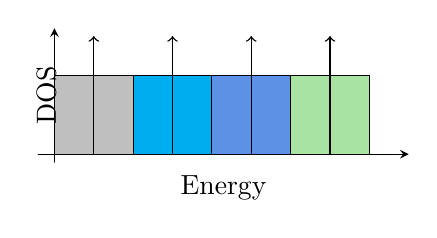
\begin{tikzpicture}[line cap=round,line join=round]
	\definecolor{grannysmithapple}{rgb}{0.66, 0.89, 0.63}
	\definecolor{unitednationsblue}{rgb}{0.36, 0.57, 0.9}
	\begin{axis}[ticks=none,
		x=1cm,y=1cm,
		axis lines=middle,
		xmin=-0.2052410812264766,
		xmax=4.5,
		ymin=-0.1,x label style={at={(axis description cs:0.5,-0.03)},anchor=north}, y label style={at={(axis description cs:-0.03,0.5)},rotate=90},
		ymax=1.6,xlabel=Energy,ylabel=DOS]
		\filldraw[draw=black,fill=lightgray] (0,0) rectangle (1,1);
		\filldraw[draw=black,fill=cyan] (1,0) rectangle (2,1);
		\filldraw[draw=black,fill=unitednationsblue] (2,0) rectangle (3,1);
		\filldraw[draw=black,fill=grannysmithapple] (3,0) rectangle (4,1);
		\draw [->,line width=0.5pt] (0.5,0) -- (0.5,1.5);
		\draw [->,line width=0.5pt] (1.5,0) -- (1.5,1.5);
		\draw [->,line width=0.5pt] (2.5,0) -- (2.5,1.5);
		\draw [->,line width=0.5pt] (3.5,0) -- (3.5,1.5);
		\draw [line width=0.5pt] (4,1)-- (4,0);
	\end{axis}
\end{tikzpicture}